%\documentclass[brudnopis]{xmgr}
% Jeśli nowe rozdziały mają się zaczynać na stronach nieparzystych:
\documentclass[openright]{xmgr}

\usepackage[utf8]{inputenc}

\definecolor{bluekeywords}{rgb}{0.13,0.13,1}
\definecolor{greencomments}{rgb}{0,0.5,0}
\definecolor{redstrings}{rgb}{0.9,0,0}
\usepackage[dvipsnames]{xcolor}

% install minted package to highlight source code
%\usepackage{minted}
%\defaultfontfeatures{Scale=MatchLowercase}
%\setmainfont[Numbers=OldStyle,Ligatures=TeX]{Minion Pro}
%\setsansfont[Numbers=OldStyle,Ligatures=TeX]{Myriad Pro}
% for fontspec version < 2.0
% \setmainfont[Numbers=OldStyle,Mapping=tex-text]{Minion Pro}
% \setsansfont[Numbers=OldStyle,Mapping=tex-text]{Myriad Pro}
%\setmonofont[Scale=0.75]{Monaco}
\usepackage{listings}
\lstloadlanguages{Ruby}
\lstset{basicstyle=\footnotesize, numbers=left, showspaces=false,showtabs=false,breaklines=true,showstringspaces=false,breakatwhitespace=true,frame=trBL, escapeinside={(*@}{@*)},
label=listing:RubyTest,
float=h,
caption=test.rb,
firstnumber=1,
language=Ruby,
keywordstyle=\color{red},
stringstyle=\color{blue},
}
\renewcommand{\lstlistlistingname}{Spis kodów źródłowych}
% Opcjonalnie identyfikator dokumentu
% drukowany tylko z włączoną opcją 'brudnopis':
\wersja   {wersja wstępna [\ymdtoday]}

\author   {Dominika Pienczyn}
\nralbumu {236\,389}
\email    {walenty@szczesny.com.pl}

\title    {System rejestrowania usterek ~ i napraw}
\date     {2017}
\miejsce  {Gdańsk}

\opiekun  {dr W. Bzyl}

% dodatkowe polecenia
%\renewcommand{\filename}[1]{\texttt{#1}}
%\definecolor{stress}{cmyk}{0,1,0.13,0} % RubineRed
%\definecolor{topic}{cmyk}{0.98,0.13,0,0.43} % MidnightBlue

\begin{document}
	
	% streszczenie
	\begin{abstract}
		Praca przedstawia aplikację internetową o nazwie ,,Awaria'', która jest systemem rejestrującym usterki oraz naprawy sprzętu. Została stworzona w grupie 3-osobowej (Kamil Pek, Marcin Dawidowski, Dominika Pienczyn). W projekcie wykonałam szatę graficzną, tak zwany frontend aplikacji. Podczas tworzenia skupiałam się na tym, aby strona dostosowana była do urządzeń mobilnych, co obecnie jest standardem. Zajmowałam się również przeprowadzaniem testów strony, które uświadomiły mi jakie elementy należy jeszcze poprawić. Zaimplementowałam elementy, które poprawiły funkcjonowanie aplikacji: automatyzacja powiadomień, filtracja danych, uaktywnienie resetowania hasła oraz e-maili powitalnych podczas rejestracji.\\ 
		\indent Do stworzenia aplikacji wykorzystano system Linux, bazę danych PostgreSQL, framework Ruby on Rails oraz Bootstrap, a następnie wdrożono ją na serwer Heroku.\\
		\indent Wgląd do szerszej dokumentacji możliwy jest pod adresem \texttt{\url{https://github.com/dpienczyn/awaria1}} i przechowywany jest w repozytorium GitHuba razem z kodem aplikacji.\\
		\indent Aplikacja dostępna jest pod adresem \texttt{\url{https://awaria-system.herokuapp.com/}}.
	\end{abstract}
	
	% słowa kluczowe
	\keywords{aplikacja internetowa, aplikacja mobilna, ruby on rails, system rejestrowania, naprawa, bootstrap, interfejs graficzny użytkownika}
	
	% tytuł i spis treści
	\maketitle
	
	% wstęp
	\introduction
	
	Graficzny interfejs użytkownika to ogólne określenie sposobu prezentacji informacji przez komputer oraz interakcji z użytkownikiem, polegające na rysowaniu i obsługiwaniu widżetów. Głównym aspektem tworzonego interfejsu jest optymalne rozmieszczenie elementów na stronie, zgodnie z ergonomią pracy oraz szatą graficzną, która pełni ważną rolę dopełniającą i pomaga prowadzić użytkowników przez strukturę informacji prezentowaną w serwisie. Kolejnym istotnym elementem jest to, aby aplikacja była responsywna. W dzisiejszym świecie korzystamy z różnego typu urządzeń nośnych tzn tabletów, smartfonów itp, dlatego tak ważne jest to, aby aplikacja umiała dopasować się do każdej rozdzielczości i każdego nośnika automatycznie. Od prawidłowo zaprojektowanego interfejsu zależy sukces strony, wygoda, intuicyjność oraz odpowiednia funkcjonalność. W mojej pracy zamierzam przedstawić to jak w prosty i skuteczny sposób można zmienić szatę graficzną aplikacji oraz kilka innych elementów, które umożliwiły zwiększenie funkcjonowania danego systemu.
	
	\chapter{Wykorzystane technologie}
	
	\section{Ruby on Rails}
	
	W utworzonym projekcie wykorzystano język Ruby wersje 2.3 oraz framework Rails wersja 5.0.0. Ruby on rails jest frameworkiem open source i wykorzystuje się go do tworzenia aplikacji webowych. Napisany został z wykorzystaniem architektury MVC \emph{(ang. Model-View-Controller)}.\\
	
	\textbf{Modele} \emph{(ang. Model)} reprezentują dane aplikacji i służą do manipulowania tymi danymi. Model odpowiada jednej tabeli w bazie danych.\\
	
	
	\textbf{Widoki} \emph{(ang. View)} tworzą interfejs użytkownika aplikacji i służą do dostarczania danych do przeglądarki internetowej, bądź innego urządzenia. Są to pliki zawierające kod w języku Ruby i HTML.\\
	
	\textbf{Kontrolery} \emph{(ang. Controller)} w nich znajduje się cała logika aplikacji. Mają za zadanie połączyć model i widok. Odpowiadają za przetwarzanie żądań przychodzących z przeglądarki internetowej, za pozyskiwanie danych z modeli oraz przekazanie ich do widoków w celu ich reprezentacji.
	\newpage
	
	\section{Bootstrap}
	
	Bootstrap, framework CSS, zawiera wiele narzędzi, które przydają się podczas tworzenia interfejsu graficznego stron oraz aplikacji internetowych. Jest bardzo prosty w obsłudze, nie potrzeba wiele umiejętności żeby zacząć z nim pracować. Wystarczy podstawowa wiedza, by rozpocząć tworzenie czegoś własnego. Bootstrap bazuje głównie na gotowych rozwiązaniach HTML i CSS. Może być używany do stylizacji m.in. przycisków, formularzy, wykresów, nawigacji oraz innych komponentów wyświetlanych na stronie. Framework korzysta również z języka JavaScripts. By zacząć korzystać z platformy Bootstrap, należy w pliku Gemfile dodać gem, który odpowiedzialny jest za odpowiednie funkcjonowanie frameworka.
	
	\begin{lstlisting}[language=Ruby,lineskip={-1pt},caption=Plik \textit{Gemfile}]
gem 'bootstrap-sass', '~> 3.3.7'
	\end{lstlisting}

	Bootstrap jest platformą stylów CSS, więc każdy kod powinien być zapisany w pliku o dowolnej nazwie z rozszerzeniem \textit{*css.scss}. Pliki musza być umieszczone w przeznaczonym do tego katalogu \textit{/app/assets/stylesheets.\textbf{}}\\	
	
	\begin{flushleft}
		Wymagane są również referencje do skryptów JavaScripts, które wykorzystywane są przez platformę.
	\end{flushleft}
	
	\begin{lstlisting}[language=Ruby,lineskip={-1pt},caption=Referencje do skryptów JavaScripts]
//= require bootstrap-sprockets
//= require bootstrap
	\end{lstlisting}
	
	\chapter{Implementacja}
	
	\section {Interfejs graficzny użytkownika}
	
	Pierwszy interfejs graficzny został stworzony w latach 70, XX wieku przez firme Xerox. Służy on do komunikowania się człowieka z oprogramowaniem komputera, wykorzystując obiekty wyświetlane na monitorze w trybie graficznym. Interfejs graficzny określa wygląd oraz funkcjonalność obiektów. \\

Składa sie zazwyczaj z:\\
	
\begin{itemize}
	\item
	menu
	
	\item
	 wyświetlanych na ekarnie ikonek, które oznaczają obiekty i polecenia
	
	\item
	okien wyświetlanych na ekranie
	\item
	funkcji dialogowych np. zapytań potwierdzajacych usunięcie lub zmiane wydanego polecenia
\end{itemize}
	
	\textbf{Projektowanie responsywne} \textit{(ang. responsive)} \cite{framework} w polskim tłumaczeniu oznacza to coś czułego, wrażliwego i ma na celu tworzenie stron internetowych, które dynamicznie adaptują się do swojego środowiska. Dzięki temu strona ma płynną, elastyczną strukturę i dopasowuje się do dowlonego urządzenia: smartfona, tableta, telewizora lub komputera. Ponadto strony responsywne, są kompatybilne z interfejsami dotykowymi urządzeń mobilnych. 
	\newpage
	\section{Panel logowania}
	
	Panel logowania użytkownika jest dla aplikacji istotnym elementem, ponieważ odbiorca wchodząc na strone zostaje automatycznie do niego przekierowany. Dlatego zadbałam o to, by strona w projekcie była atrakcyjna graficznie, a zarazem prosta w obsłudze. Główną zasadą, której trzymałam się podczas tworzenia frontendu była estetyka oraz niezróżnicowany wygląd aplikacji.  
	
	Wygląd panelu logowania przed ostylowaniem kodem HTML wyglądał przeciętnie, zawierał tylko jedną klase \textit{div class="field"}. Format panelu został przedstawiony poniżej:
	
	\begin{figure}[!tbh]
		\centering
		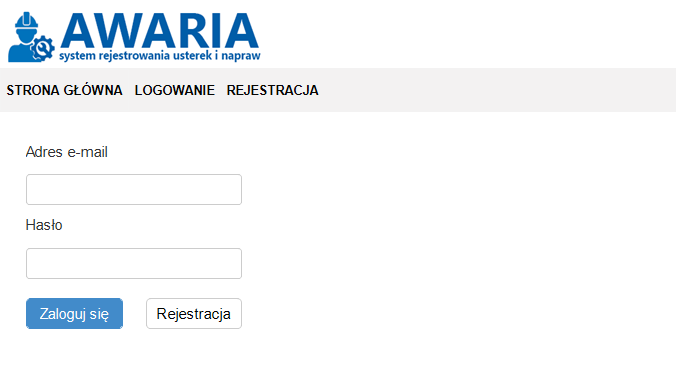
\includegraphics[width=\linewidth]{image/panel}
		\caption{Panel logowania przed ostylowaniem kodem HTML}
	\end{figure}
	
	\newpage
	\begin{lstlisting}[language=Ruby,lineskip={-1pt},caption=Kod odpowiedzialny za panel logowania]
<div class="field">
  <%= f.label :email %><br/>
  <%= f.email_field :email, autofocus: true %>
</div>
<div class="field">
  <%= f.label :password %><br/>
  <%= f.password_field :password, autocomplete: "off" %>
</div>
	\end{lstlisting}
	
	\begin{figure}[!tbh]
		\centering
		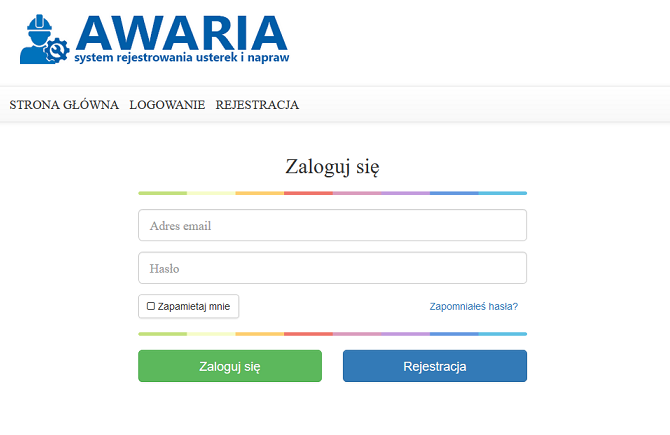
\includegraphics[width=\linewidth]{image/panelhtml}
		\caption{Ostylowany panel logowania}
	\end{figure}
\newpage
	\begin{lstlisting}[language=Ruby,lineskip={-1pt},caption= Kod obudowany kodem HTML]
<div class="container">
<div class="row">
<div class="col-xs-12 col-sm-8 col-md-6 col-sm-offset-2 col-md-offset-3">
<fieldset>
<h2 class="text-center">Zaloguj się</h2>
<hr class="colorgraph">
<div class="form-group">
  <%= f.email_field :email, autofocus: true, class: "form-control input-lg", placeholder: "Adres email" %>
</div>
<div class="form-group">
  <%= f.password_field :password, autocomplete: "off", class: "form-control input-lg", placeholder: "Haslo"  %>
</div>
	\end{lstlisting}

W kodzie zastosowano poniższą klase \textbf{\textit{div class="col-xs-12 col-sm-8 col-md-6 col-sm-offset-2 col-md-offset-3"}}, dzięki której uzyskujemy efekt strony responsywnej \cite{css} i możliwej do obejrzenia na dowolnym wyświetlaczu:
\begin{itemize}
	\item
\textit{col-xs} stosuje się dla bardzo małych wyświetlaczy (szerokość ekranu mniejsza niż 768 pikseli)
\item
\textit{col-sm} stosuje się dla małych wyświetlaczy (szerokość ekranu większa równa 768 pikseli)
\item
\textit{col-md} stosuje się dla średnich wyświetlaczy (szerokość ekranu wieksza, równa 992 pikseli)\\
\end{itemize}

Klasy służące do przesuwania kolumn względem siebie, służą do zwiększenia odstępu po lewej stronie kolumny:
\begin{itemize}
\item
\textit{col-sm-offset-2} w przypadku stron dla małych wyświetlaczy, jeżeli chcemy przenieść kolumnę obejmującą dwie kolumny w prawą strone
\item
\textit{col-md-offset-3} w przypadku stron dla średnich wyświetlaczy, jeżeli chcemy przenieść kolumnę obejmującą trzy kolumny w prawą strone
\end{itemize}

\indent Aby była możliwość tworzenia rzędów, to \textbf{\textit{div class="col-xs-12 col-sm-8 col-md-6 col-sm-offset-2 col-md-offset-3"}} musi zostać umieszczony w kontenerze \textit{div class="container"} oraz wewnątrz kontenera musi znaleźć się klasa \textit{div class="row"}.\\

Klasa \textit{form-group} służy do tworzenia formularzy, natomiast klasa \textit{class: "form-control input-lg"} znajdująca się pomiedzy znacznikami kodu Ruby sprawia, że element rozciaga się na całą dostępną szerkość ekranu.

W pliku CSS odnosimy sie do styli klasy  \textit{hr class="colorgraph"} w której określamy rozmiar wysokości obszaru \textit{(height)}, cechy górnego obramowania \textit{(border-top)} lub ustawiamy kolor tła elementu \textit{(background)}.
\begin{lstlisting}[language=Ruby,lineskip={-1pt},caption=Kod CSS dla panelu logowania]
.colorgraph {
border-top: 70px;
height: 5px;
border-top: 0;
background: #c4e17f;
border-radius: 5px;
}
\end{lstlisting}

W panelu logowania wykorzystano kod JavaScript obsługujący element \textit{checkbox}.\\

\begin{figure}[!tbh]
	\centering
	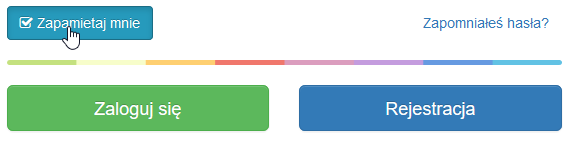
\includegraphics[width=\linewidth]{image/checkbox}
	\caption{Checkbox w panelu logowania}
\end{figure}	
	
	\section{Tabela zgłoszeń}
	
	Tabela zgłoszeń, po wygenerowniu kodu nie posiadała przycisków. Jej kolumny i wiersze nie były oddzielone linią w żaden sposób. Pod wpływem zmniejszania obrazu, tabela nie dopasowywała się do narzuconej jej rozdzielczości, czego efektem był brak możliwości odczytu niektórych danych, znajdujących sie w tabelce. 
	
	\begin{figure}[!tbh]
		\centering
		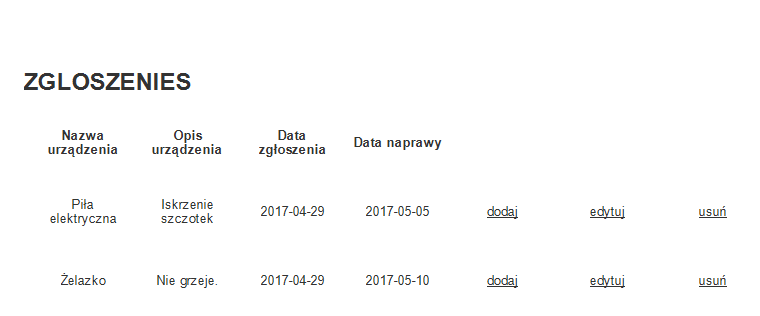
\includegraphics[width=\linewidth]{image/zgloszenie}
		\caption{Tabela zgłoszeń po wygenerowaniu kodu}
	\end{figure}

	Do stworzenia tabelki wykorzystano klasę \textit{div class="table-responsive"}, dzięki której tabela zamyka się w kontenerze z poziomym paskiem przewijania podczas mniejszych rozdzielczości.
		
	\begin{figure}[!tbh]
		\centering
		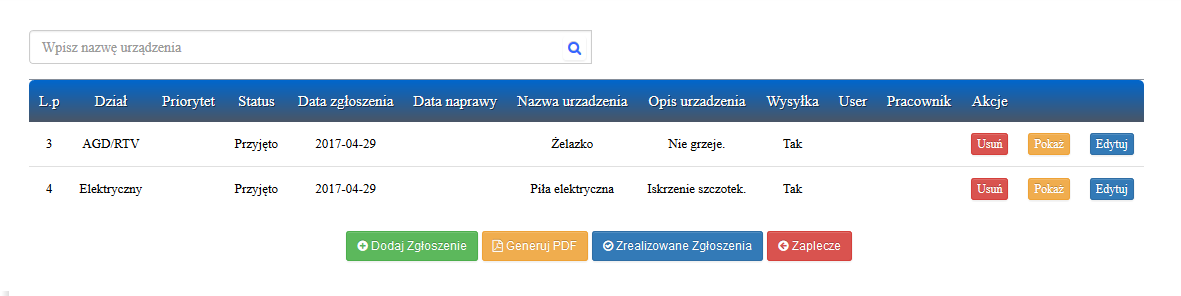
\includegraphics[width=\linewidth]{image/tabelka}
		\caption{Ostylowana kodem HTML tabela zgłoszeń}
	\end{figure}
	
	\begin{lstlisting}[language=Ruby,lineskip={-1pt},caption=Element klikalny]
<%= link_to('Usun', zgloszeny, method: :delete, data: { confirm: 'Jestes pewny?' }, class:'btn btn-danger btn-xs') %>
	\end{lstlisting}
	
	Do stworzenia przycisku należało użyć klasy \textit{btn}. W klasie widzimy również \textit{btn-danger}, dzięki czemu element klikalny jest koloru czerwonego oraz \textit{btn-xs} co określa wielkość przycisku w tym przypadku jest to element bardzo mały. 
	
	\chapter{Elementy funkcjonalne systemu}
	
	\section{Uaktywnienie przypominania hasła na e-mail}
	
	Konfiguracji przpominania hasła na adres e-mail użytkownika \cite{configuration}, dokonuje się w pliku konfiguracyjnym \textit{config/environments/production.rb.} Ze względu na wdrożenie aplikacji na serwer Heroku, wykorzystałam dodatkowy element tej platformy do korespondencji z użytkownikiem o nazwie Sendgrid.  
	
	\begin{lstlisting}[language=Ruby,lineskip={-1pt},caption=Konfiguracja pliku \textit{production.rb}]
config.action_mailer.smtp_settings = {
user_name: ENV['SENDGRID_USERNAME'],
password: ENV['SENDGRID_PASSWORD'],
domain: 'awaria-system.herokuapp.com',
address: 'smtp.sendgrid.net',
port: 587,
authentication: :plain,
enable_starttls_auto: true
}
	\end{lstlisting}
	
	W pliku, dane na temat hasła oraz nazwy użytkownika, zostały ukryte i dostępne są tylko dla użytkowników do tego uprawnionych. Wszystkie dane znajdują się na platformie Heroku. W sekcji \textit{domain} deklarujemy adres url strony pod który została wdrożona.
	\newpage
	\section{Uaktywnienie e-maili powitalnych podczas rejestracji}
	
	W pracy wykorzystałam element e-maili powitalnych, podczas pierwszej wizyty na stronie, które informują użytkownika o pozytywnym przejściu rejestracji. Wiadomości powitalne wysyłane są automatycznie, tuż po aktywacji adresu mailowego. Są elementem podtrzymania dalszej komunikacji z klientem. Do zaimplementowania tej funkcjonalności wykorzystałam plik \textit{app/models/user.rb.} 
	
	\begin{lstlisting}[language=Ruby,lineskip={-1pt},caption=Kod odpowiedzialny za wysyłanie e-mail powitalnych]
class User < ApplicationRecord
  after_create :welcome_send
  def welcome_send
	WelcomeMailer.welcome_send(self).deliver
  end
	\end{lstlisting}
	
	W treści wiadomości, na adres użytkownika zostaje wysłane hasło, wprowadzone podczas rejestracji oraz logo firmy \cite{api}. Wiadomości przesłane zostają w formie \textit{html} oraz \textit{txt.} Wybrałam te dwa formaty, ponieważ \textit{txt} z pewnością trafi do każdego odbiorcy, natomiast wiadomości w formie \textit{html} mogą być nieczytelne dla niektórych przeglądarek pocztowych. Różnica polega na tym, że dzięki kodzie HTML wiadomości wyglądają atrakcyjniej graficznie.
	Treści wiadomości powitalnych w formie \textit{.html} oraz \textit{.txt} zostały zawarte w pliku \textit{app/views/welcome\_mailer.}
	
	Na kolejnej stronie można zobaczyć, jak graficznie prezentują się wiadomości powitalne oraz jaką zawierają treść. 
	\newpage
	\begin{figure}[!tbh]
		\centering
		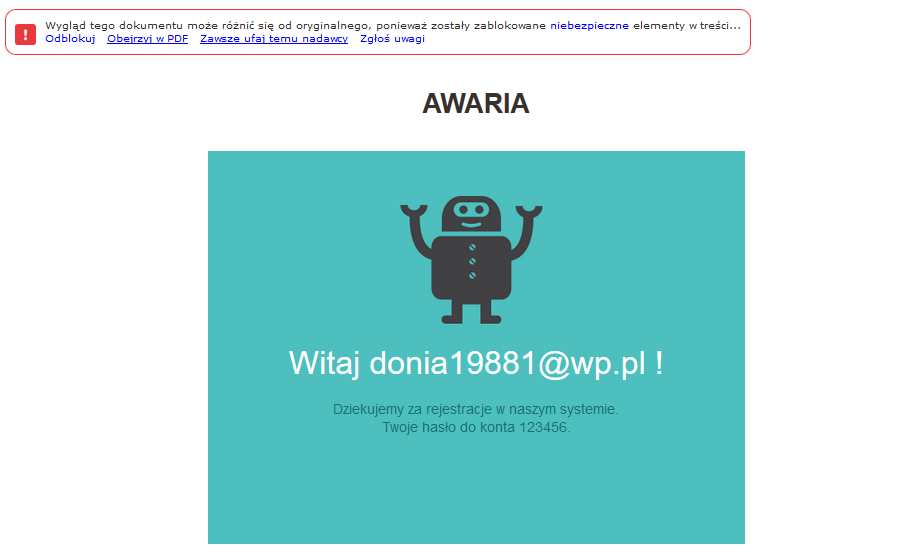
\includegraphics[width=\linewidth]{image/emailhtml}
		\caption{Format \textit{.html}}
	\end{figure}


	\newpage
	\section{Przeszukiwanie danych w czasie rzeczywistym}
	
	W aplikacji wykonano dodatkowo przeszukiwanie danych w czasie rzeczywistym \cite{filtrowanie}, umożliwiające wyszukanie danych w tabeli. Używając filtru, można wyświetlić tylko dane, które nas interesują i ukryć pozostałe. Po przefiltrowaniu danych w zakresie tabel można ponownie zastosować filtr w celu otrzymania aktualnych danych, badź można wyczyścić filtr w celu ponownego wyświetlenia wszystkich danych w tabeli. 
	Filtr, który zastosowałam w projekcie został stworzony dla tabel: użytkownika, stanowiska, działu, zgłoszeń. W przeszukiwniu danych dla jednej tabeli, zastosowałam kilka warunków. Podczas wpisywania fraz, program nie rozróżnia wielkości liter za co odpowiada operator ILIKE .\\
	
	\textbf{Tabela użytkowników, filtrowanie według:}\\
	\textendash\space imię \textit{(ang. first\_name)}\\
	\textendash\space nazwisko \textit{(ang. last\_name)}\\
	\textendash\space adres e-mail
	\textit{(ang. email)}\\
	
	\textbf{Tabela zgłoszeń, filtrowanie według:}\\
	\textendash\space nazwa urządzenia\\
	\textendash\space adres e-mail\\
	\textendash\space imię
	\textit{(ang. first\_name)}\\
	\textendash\space nazwisko
	\textit{(ang. last\_name)}\\
	
	\textbf{Tabela stanowisk, filtrowanie według:}\\
	\textendash\space nazwa\\
	
	\textbf{Tabela działów, filtrowanie według:}\\
	\textendash\space nazwa\\
	
	Do wykonania tego elementu funkcjonalnego, wykorzystałam plik\\
	\textit{app/controllers/zgloszenies\_controller.rb.}
	
	\begin{lstlisting}[language=Ruby,lineskip={-1pt},caption=Dane według których nastepuje przeszukiwanie]
@zgloszenies = Zgloszenie.includes(:user)
.where("zgloszenies.nazwa_urzadzenia ILIKE :q OR users.email ILIKE :q OR users.first_name ILIKE :q OR users.last_name ILIKE :q", 
q: "%#{params[:search]}%").references(:users)
	\end{lstlisting}
	
	W tym pliku zostały zawarte wszystkie dane, które umożliwiają przeszukanie tabeli ,,zgłoszenie''. Referencje użytkownika zostały powiązane z tabelą zgłoszeń, co umożliwia nie tylko wyszukanie interesującego nas zgłoszenia, jak również na podstawie zgłoszeń możemy wyszukać w bazie użytkownika oraz sprawdzić jakie zgłoszenie złożył i w jakim czasie.
	Funkcjonowanie przeszukiwania danych w czasie rzeczywistym opiera się także na kodzie JavaScript:\\
	
	\textit{app/assets/javascripts/custom.js}
	\begin{lstlisting}[language=Ruby,lineskip={-1pt},caption=JavaScripts - przeszukiwanie w czasie rzeczywistym]
$(document).on('keyup', '.search_form_z input', function() {
  $('.search_form_z').delay(200).submit();
});
	\end{lstlisting}
	
	Dzięki wykorzystanemu kodzie JavaScripts użytkownik podczas wpisywania frazy nie musi dodatkowo klikać na przycisk, proces odbywa się w momencie, kiedy w wyszukiwarke zostaje wprowadzona pierwsza litera. Czas wyszukiwania to 200 milisekund. 
	\newpage
	\section{Automatyzacja powiadomień}
	
	W projekcie utworzyłam automatyzacje powiadomień, która jest w stałym kontakcie z użytkownikiem zgłaszającym usterkę w systemie. Poprzez rejestrację w systemie, za pomocą adresu e-mail, na ten sam adres otrzymuje powiadomienia zawierające aktualny status swojego produktu. Na powiadomienia składają się trzy etapy:
	
	\begin{itemize}
		\item
		\textbf{started} \textit{(przyjęcie usterki)} etap na którym, następuje zgłoszenie usterki w systemie
		
		\item
		\textbf{inprogress} \textit{(rozpoczęcie naprawy)} etap na którym, rozpoczyna się naprawę usterki
		
		\item
		\textbf{finished} \textit{(zakończenie naprawy)} etap na którym, zakończono naprawę usterki
	\end{itemize}
	
	Do zaimplementowania tego elementu wykorzystałam plik znajdujący się w \textit{app/mailers/customer\_notification\_mailer.rb} w którym zawarłam kod:
	
	\begin{lstlisting}[language=Ruby,lineskip={-1pt},caption=Opis statusów w modelu]
class CustomerNotificationMailer < ApplicationMailer
  def started(zgloszenie_id, user_id)
	@zgloszenie = Zgloszenie.find(zgloszenie_id)
	user = User.find(user_id)
	mail(subject: default_i18n_subject, to: user.email) 
  end
	\end{lstlisting} 
	
	W pliku \textit{zgłoszenies\_controller.rb} znajdujący się w ścieżce
	\textit{app/controllers} znjadują się kody:
	
	\begin{lstlisting}[language=Ruby,lineskip={-1pt},caption=Powiadomienia o przyjęciu usterki do naprawy]
def create
  CustomerNotificationMailer.started(@zgloszeny.id, @zgloszeny.user_id).deliver_later
end
	\end{lstlisting}
	
	Metoda \textit{def create} odpowiada za tworzenie nowych zgłoszeń do której przypisano status \textit{started}.
	
	\begin{lstlisting}[language=Ruby,lineskip={-1pt},caption=Powiadomienia o rozpoczeciu i zakończeniu naprawy usterki]
def update
  CustomerNotificationMailer.send(@zgloszeny.status, @zgloszeny.id, @zgloszeny.user_id).deliver_later if !@zgloszeny.started?
end
	\end{lstlisting}
	
	Metoda \textit{def update} odpowiada za edycję zgłoszeń do której przypisano status \textit{inprogress} i \textit{finished}.
	
	\chapter{Testowanie aplikacji na urządzeniach mobilnych}
	
	Test optymalizacji mobilnej jest jedną z wielu rzeczy, które są bardzo istotne a z tego względu że więcej osób na dzień dzisiejszy korzysta z internetu za pomocą urządzeń mobilnych. 

	Aby strona nadawała się do użytku na urządzeniach mobilnych trzeba pamietać o tym by:
	
	\begin{itemize}
		\item Czcionka nie była zbyt mała, ponieważ strona staje się nieczytelna i wymaga powiekszenia widoku w celu odczytania jej treści.
		\item Elementy dotykowe, czyli przyciski i linki nawigacyjne, nie były zbyt blisko siebie, ponieważ użytkownicy korzystając z takiej strony mają problemy z naciśnięciem wybranego elementu, bez dotknięcia elementu sąsiadującego.
		\item Jeżeli rozmiar zawartości jest niedopasowany do widocznego obszaru, należy upewnić się czy strona korzysta z wartości względnych szerokości i pozycji elementów css. Ważne jest również to, by obrazy się skalowały.
	\end{itemize}
	
	\newpage
	Aby przeglądarka odpowiednio przeskalowała zaprojektowaną stronę do rozmiarów okna w pliku \textit{app/views/layouts/application.html.erb} należy dodać meta-tag \cite{framework}:
	
	\begin{lstlisting}[language=Ruby,lineskip={-1pt},caption=Meta tag odpowiedzialny za skalowanie]
<meta name="viewport" content="width=device-width, initial-scale=1.0">
	\end{lstlisting}
	
	Testy na optymalizacje mobilną, wykonałam za pomocą narzędzia \textbf{Mobile Friendly Test Google Search Console}.
	
	\begin{figure}[!tbh]
		\centering
		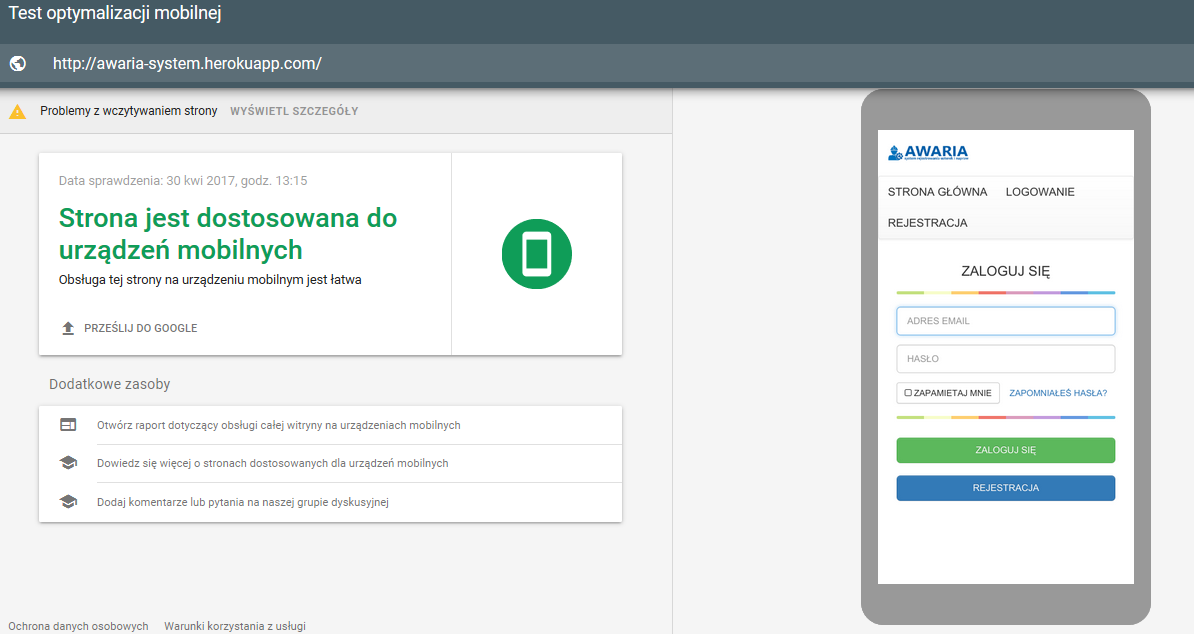
\includegraphics[width=\linewidth]{image/testm}
		\caption{Test optymalizacji mobilnej}
	\end{figure}
	
	\chapter{Test szybkości ładowania strony}
	Test szybkości ładowania strony polega na zbadaniu w jakim czasie ładuje się aplikacja. Im krótszy czas tym wyższa pozycja w Google. Według przeprowadzonych badań, im wolniej ładuje się strona, tym mniej czasu spędza na niej użytkownik. Wywiera także istotny wpływ na przeglądanie podstron przez użytkownika i szybkie dotarcie przez niego do porządanych informacji. Przekłada się to na oszczędność czasu oraz oszczedność transferu w przypadku urządzeń mobilnych. Dzięki szybko działającej stronie, roboty wyszukiwarek mogą szybciej przeskanować strone i wyszukać nowe treści.
	
	Po wykonaniu testów, narzędzie wskazało obszary, w których miejscach należałoby użyć udoskonaleń by strona ładowała się o wiele szybciej. Obszary dzielone są według trzech priorytetów: wysokim (\textit{kolor czerwony}), średnim (\textit{kolor żółty}), niskim (\textit{kolor zielony}).
	
	Według \textbf{PageSpeed Insights}, stronę można uznać za działającą dobrze, kiedy wynik w obu testach osiągnie conajmniej 85 punktów.\\
	
	\newpage
	Na podstawie badań \textbf{PageSpeed Insights} aplikacja otrzymała następujące wyniki: 	
	
	\begin{figure}[!tbh]
		\centering
		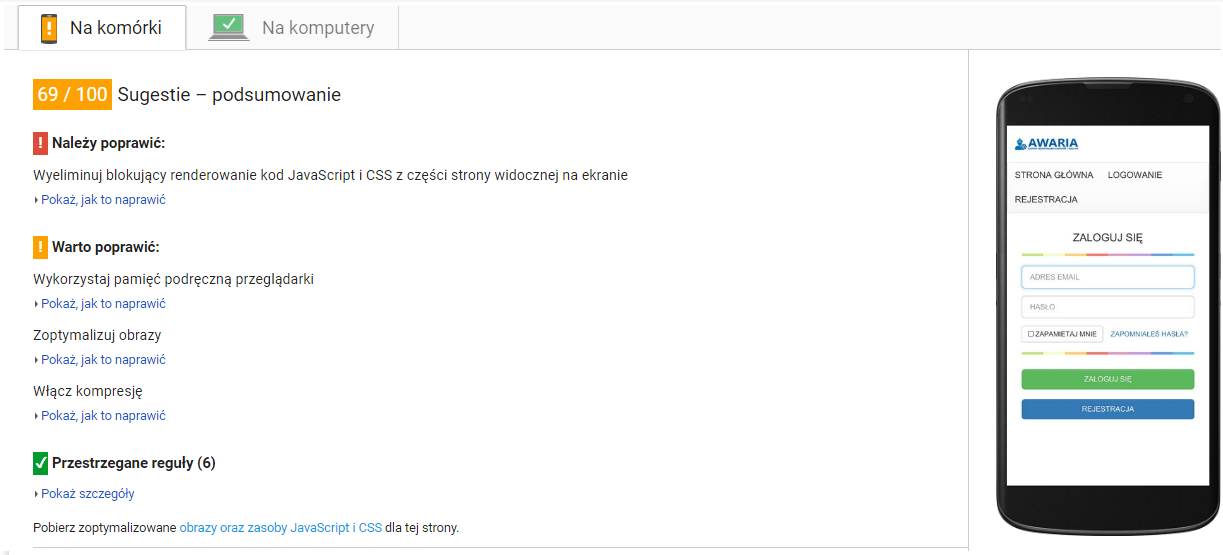
\includegraphics[width=\linewidth]{image/phoneo}
		\caption{Wynik szybkości działania strony na urządzeniach mobilnych}
	\end{figure}
	
	\begin{figure}[!tbh]
		\centering
		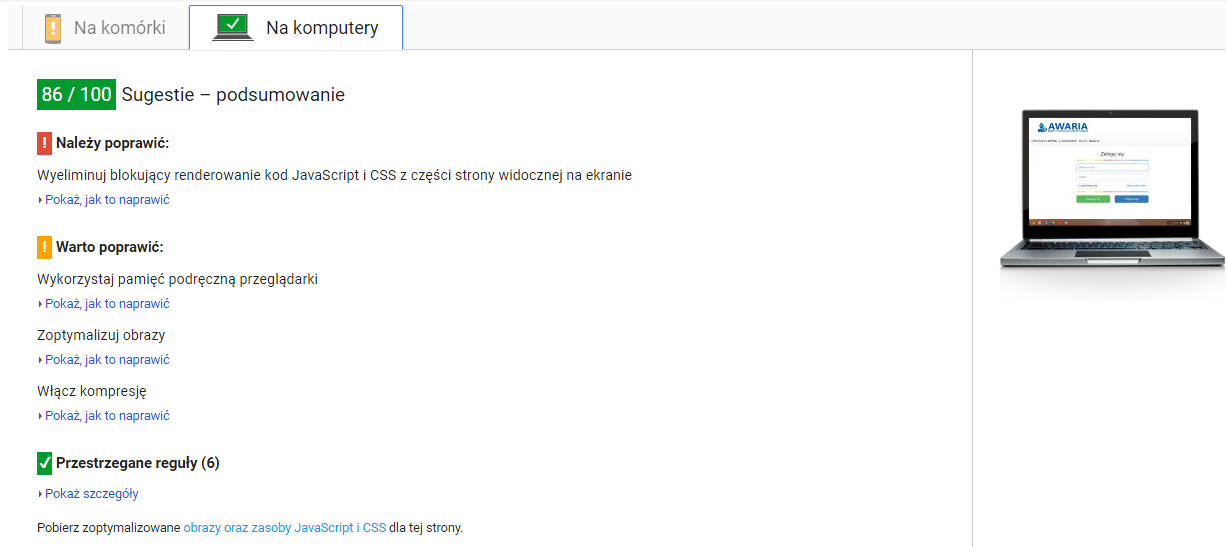
\includegraphics[width=\linewidth]{image/computero}
		\caption{Wynik szybkości działania strony na komputerze}
	\end{figure}
	\newpage
	Podczas wykonywania testów, aplikcja otrzymała kilka sugesti w celu poprawienia jakości, szybkości strony. W tabeli w punktach, wyszczególniono elementy, na które składa się szybsze ładowanie strony.
	
	\begin{table} [!h]
		\centering
		\begin{footnotesize}
			\caption{Podsumowanie}
	\begin{tabular}{|c|c|c|}
		\hline  & Komputer  & Telefon \\ 
		\hline  Skróć czas odpowiedzi serwera &  &  \\ 
		\hline  Wyeliminuj blokujący renderowanie kod JavaScript i CSS &  &  \\ 
		\hline Wykorzystaj pamięć podręczną przeglądarki &  &  \\ 
		\hline Zoptymalizuj obrazy &  &  \\ 
		\hline Włącz kompresję &  &  \\ 
		\hline Nadaj priorytet widocznej treści & tak & tak \\ 
		\hline Unikaj przekierowań stron docelowych & tak & tak \\ 
		\hline Zmniejsz CSS & tak & tak \\ 
		\hline Zmniejsz HTML & tak & tak \\ 
		\hline Zmniejsz JavaScript & tak & tak \\ 
		\hline 
	\end{tabular}
\end{footnotesize}
\end{table}

	
	\begin{figure}[!tbh]
		\centering
		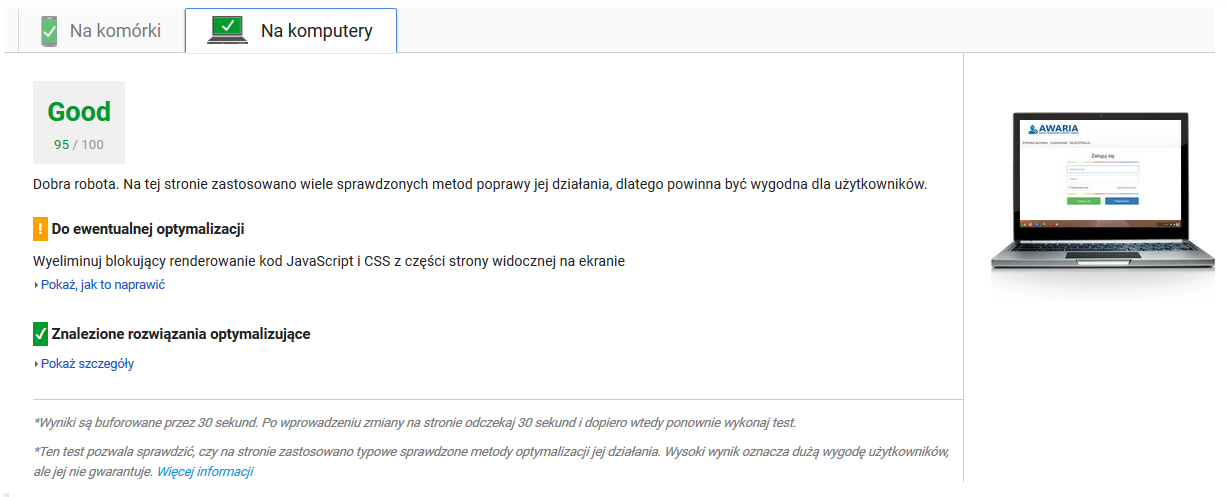
\includegraphics[width=\linewidth]{image/computerr}
		\caption{Wynik szybkości działania strony na komputerze po naprawie błędów}
	\end{figure}
	
	\begin{figure}[!tbh]
		\centering
		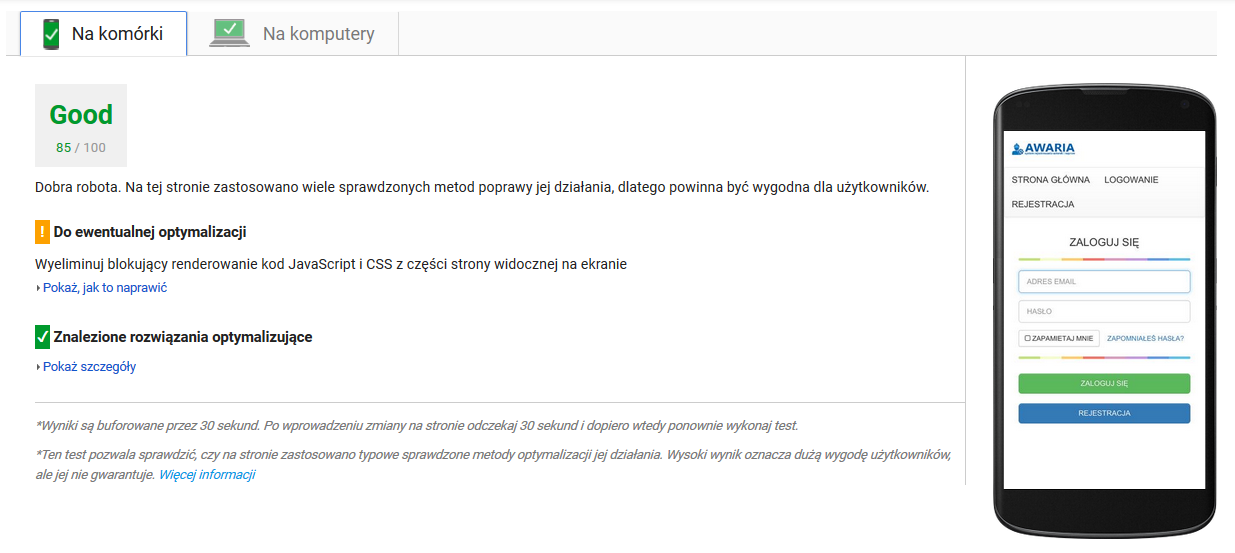
\includegraphics[width=\linewidth]{image/phonee}
		\caption{Wynik szybkości działania strony na telefonie po naprawie błędów}
	\end{figure}
	\newpage
	
	Po optymalizacji błędów, strona na komputer i telefon uzyskła więcej punktów. Tabelka, po optymailizacji błędów prezentuje się następująco. 
	
	\begin{table} [!h]
		\centering
		\begin{footnotesize}
			\caption{Podsumowanie po naprawie błędów}
			\begin{tabular}{|c|c|c|}
				\hline  & Komputer  & Telefon \\ 
				\hline  Skróć czas odpowiedzi serwera & tak & tak \\ 
				\hline  Wyeliminuj blokujący renderowanie kod JavaScript i CSS &  &  \\ 
				\hline Wykorzystaj pamięć podręczną przeglądarki & tak & tak \\ 
				\hline Zoptymalizuj obrazy & tak & tak \\ 
				\hline Włącz kompresję & tak & tak \\ 
				\hline Nadaj priorytet widocznej treści & tak & tak \\ 
				\hline Unikaj przekierowań stron docelowych & tak & tak \\ 
				\hline Zmniejsz CSS & tak & tak \\ 
				\hline Zmniejsz HTML & tak & tak \\ 
				\hline Zmniejsz JavaScript & tak & tak \\ 
				\hline 
			\end{tabular} 
		\end{footnotesize}
	\end{table}
	
	
	\chapter{Walidacja kodu}
	
	Walidacja to inaczej proces weryfikowania poprawności składniowej pliku XHTML. Wyróżnia się dwa rodzaje takiej poprawności składniowej: połączone z kontrolą zgodności z oficjalną specyfikacją XHTML, gdzie zastosowane zostają serwisy sieciowe, tzw. parasery oraz sprawdzanie wyłącznie poprawności składniowej. W tym przypadku stosuje się specjalne programy do tego przeznaczone, czyli walidatory.\\
	
	\textit{Dlaczego zatem należy używać walidacji ?}
		\begin{itemize}
			\item Ponieważ, jeżeli kod strony jest poprawny to prawdopodobieństwo, że strona będzie dobrze wyświetlana na większości przeglądarek jest większa.
			\item Gdy strona nie zawiera błędów, to szybciej się ładuje, gdyż nie musi zastanawiać się jak interpretować nie właściwie zamieszczone znaczniki.
			\item Możliwość wykrycia i poprawy błedów przed oddaniem strony do użytku.
			\item Dzięki walidacji możemy nabyć dodatkowej wiedzy o języku XHTML oraz w przypadku zmiany specyfikacji.
		\end{itemize}
		
		Do walidacji kodu użyłam narzędzia dostępnego online o nazwie \textbf{W3C} znajdującego się pod adresem \texttt{\url{https://validator.w3.org}}.
	
	Wyniki walidacji wykazały niewielką ilość popełnionych błędów, co nie oznacza że nie należy ich wyeliminować:
	
	\begin{figure}[!tbh]
		\centering
		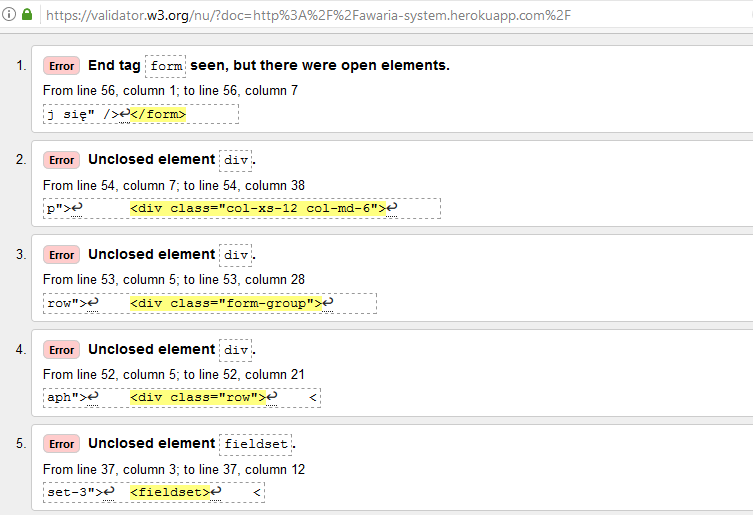
\includegraphics[width=\linewidth]{image/walidacja}
		\caption{Wynik walidacji przed naprawą błędów}
	\end{figure}
	
	\begin{figure}[!tbh]
		\centering
		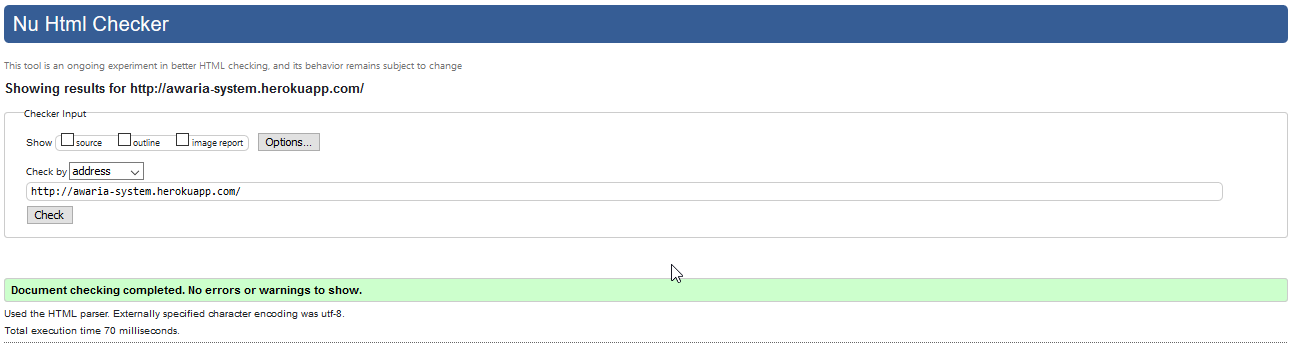
\includegraphics[width=\linewidth]{image/walidacjaa}
		\caption{Wynik walidacji po naprawie błędów}
	\end{figure}
	
	
	% zakończenie
	\summary
	Tworzenie aplikacji w Ruby on Rails sprawiło, że nabyłam kolejne, nowe umiejetności.  Nauczyłam się tworzenia elementów funkcjonalnych, nadawania szaty graficznej, testowania oraz dopasowywania strony do różnej rozdzielczości. Mam nadzieje, że nabyte umiejętności wykorzystam w kolejnym, samodzielnym projekcie, który zamierzam zrealizować w najbliższym czasie.   
	
	% załączniki (opcjonalnie):
	\appendix
	\chapter{Tytuł załącznika jeden}
	
	Treść załącznika jeden.
	
	\chapter{Tytuł załącznika dwa}
	
	Treść załącznika dwa.
	
	% literatura (obowiązkowo):
	\begin{thebibliography}{11}
		\bibitem{framework} Syed Fazle Rahman, \emph{Bootstrap. Tworzenie interfejsów stron WWW. Technologia na start!}, Wydawnictwa Helion, 2015.
		\bibitem{ror} John Elder, \emph{Ruby on Rails. Tworzenie aplikacji WWW.}, Wydawnictwa Helion, 2016.
		\bibitem{ruby} Noel Rappin, \emph{Professional Ruby on Rails.}, Wydawnictwa Wrox, 2008.
		\bibitem{api}
		Ruby on Rails API. \texttt{\url{http://api.rubyonrails.org/}} \\(Listopad 20, 2016).
		\bibitem{bootstrap}
		Kurs frameworka Bootstrap. \texttt{\url{https://kursbootstrap.pl/}} \\(Grudzień 2, 2016).
		\bibitem{html}
		Strona zawierająca kody HTML/CSS/JS. \texttt{\url{http://bootsnipp.com/}} \\(Grudzień 2, 2016).
		\bibitem{search}
		Search and Filter Rails Models Without Bloating Your Controller. \\\texttt{\url{http://www.justinweiss.com/articles/search-and-filter-rails-models-without-bloating-your-controller/}} \\(Grudzień 2, 2016).
		\bibitem{delivery}
		Action Mailer Basics. \\\texttt{\url{http://guides.rubyonrails.org/action_mailer_basics.html}} \\(Grudzień 2, 2016).
		\bibitem{configuration}
		Konfiguracja pliku production.rb. \\\texttt{\url{http://wbzyl.inf.ug.edu.pl/rails4/mail}} \\(Grudzień 2, 2016).
		\bibitem{css}
		Kurs CSS. \\\texttt{\url{http://webkod.pl/}} \\(Grudzień 2, 2016).
		\bibitem{e-mail}
		Open Source Email Templates. \\\texttt{\url{https://www.sendwithus.com/resources/templates/neopolitan}} \\(Grudzień 2, 2016).
		\bibitem{filtrowanie}
		Search, Sort, Paginate with AJAX. \\\texttt{\url{http://railscasts.com/episodes/240-search-sort-paginate-with-ajax?view=asciicast}} \\(Grudzień 2, 2016).
	\end{thebibliography}
	
	% spis rysunków (jeżeli jest potrzebny):
	\listoffigures
	
	\lstlistoflistings
	\addcontentsline{toc}{chapter}{Spis kodów źródłowych}%
	
	% spis tabel (jeżeli jest potrzebny):
	\listoftables
	
	\oswiadczenie
	
\end{document}